
% JuliaCon proceedings template
\documentclass{juliacon}
\setcounter{page}{1}

%%---- definition of custom commands
\newcommand{\abs}[1]{\left|#1\right|}
\newcommand{\vb}{\boldsymbol}
%%----

\begin{document}

% **************GENERATED FILE, DO NOT EDIT**************

\title{My JuliaCon proceeding}

\author[1]{1st author}
\author[1, 2]{2nd author}
\author[2]{3rd author}
\affil[1]{University}
\affil[2]{National Lab}

\keywords{Julia, Optimization, Game theory, Compiler}

\hypersetup{
pdftitle = {My JuliaCon proceeding},
pdfsubject = {JuliaCon 2022 Proceedings},
pdfauthor = {1st author, 2nd author, 3rd author},
pdfkeywords = {Julia, Optimization, Game theory, Compiler},
}



\maketitle

\section{Summary}
% from the JOSS docs:
% The paper should include a summary describing the high-level functionality and purpose of the software for a diverse, non-specialist audience.

%=== What is Peridynamics? ===%
\begin{figure}
\centerline{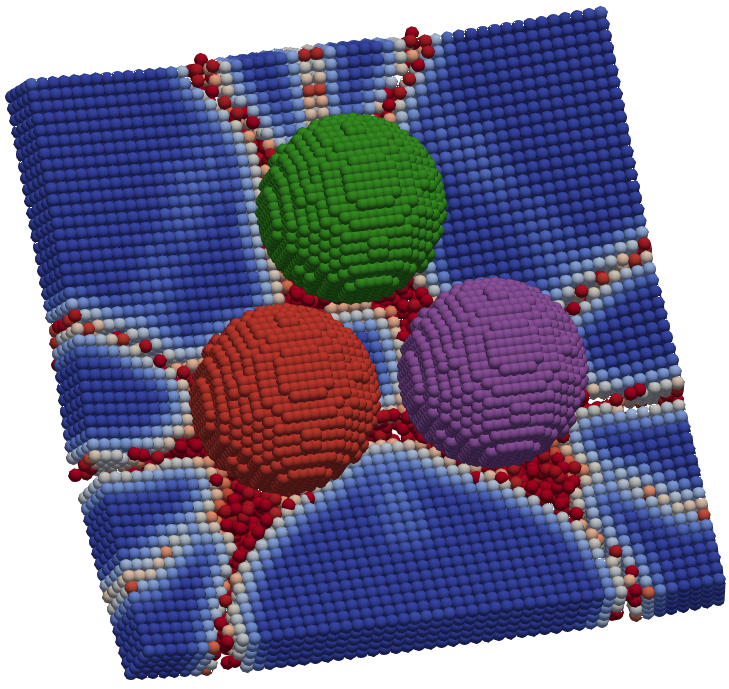
\includegraphics[width=0.8\linewidth]{logo.png}}
\caption{High-velocity contact simulation of three spheres crashing into a rectangular panel; logo of Peridynamics.jl}
\label{fig:logo}
\end{figure}

%- General peridynamics context
Peridynamics is a nonlocal continuum mechanics formulation, which was invented by Silling \cite{Silling2000}.
It has gained increased popularity as an approach for modeling fracture.
The material behavior is described by integro-differential equations that are also fulfilled for discontinuities, making it very capable of modeling crack propagation and fragmentation with large displacements.
Much peridynamics research has been done in recent years, summarized in various review papers and books \cite{Diehl2019,Javili2019Review,Madenci2014}.

%- Peridynamics short introduction
Typically, in peridynamics the continuum is discretized by material points.
Points interact only with other points inside of their specified \emph{neighborhood} or \emph{point family}~$\mathcal{H}$, which is defined as the set of points inside a sphere with the radius $\delta$, also named the \emph{horizon}.
The interaction of the point $\vb{X}$ with its neighbor $\vb{X}'$ is called \emph{bond} and defined as
\begin{equation}
\vb{\Delta X} = \vb{X}' - \vb{X} \; .
\end{equation}
The equation of motion reads
\begin{equation}
\varrho \, \vb{\ddot{u}}(\vb{X},t) = \vb{b}^{\mathrm{int}}(\vb{X},t) + \vb{b}^{\mathrm{ext}}(\vb{X},t) \; ,
\end{equation} 
with the mass density $\varrho$, the point acceleration vector $\vb{\ddot{u}}$, and the point force density vectors $\vb{b}^{\mathrm{int}}$ and $\vb{b}^{\mathrm{ext}}$.
Various formulations of peridynamics exist for the calculation of the internal force density $\vb{b}^{\mathrm{int}}$, and all of them are based on the nonlocal interactions between material points.

%- Some information on peridynamic material models
In the first original bond-based formulation (BB) of peridynamics, the internal force density is calculated by
\begin{equation}
\vb{b}^{\mathrm{int}}(\vb{X},t) = \int_\mathcal{H} \vb{f}(\vb{\Delta X}, t) \; \mathrm{d}V' \; ,
\end{equation}
with the \emph{pairwise force function} $\vb{f}$.
The BB model has intrinsic limitations due to a restriction on the Poisson's ratio \cite{Silling2007,Trageser2020}.
To overcome these restrictions, state-based peridynamics was established.
In state-based Peridynamics, the deformation states of neighboring points also influence the internal force density \cite{Silling2007}.
The general internal force density for state-based peridynamics is defined as
\begin{equation}
\vb{b}^{\mathrm{int}} (\vb{X},t) = \int_\mathcal{H} \vb{t} - \vb{t}' \; \mathrm{d}V' \; ,
\end{equation}
with the force vector states $\vb{t}=\vb{t}(\vb{\Delta X}, t)$ and $\vb{t}'=\vb{t}(-\vb{\Delta X}, t)$.
State-based peridynamics can be divided in two subcategories.
In ordinary state-based peridynamics, the force vector state $\vb{t}$ is always parallel to the deformed bond.
Non-ordinary state-based formulations do not have this restriction.
Within the local continuum consistent correspondence formulation of non-ordinary state-based peridynamics, an elastic model from the classical material theory can be used to calculate the internal force density.
Other formulations of peridynamics exist, such as continuum-kinematics-inspired peridynamics \cite{Javili2019}.

\begin{figure}
\centerline{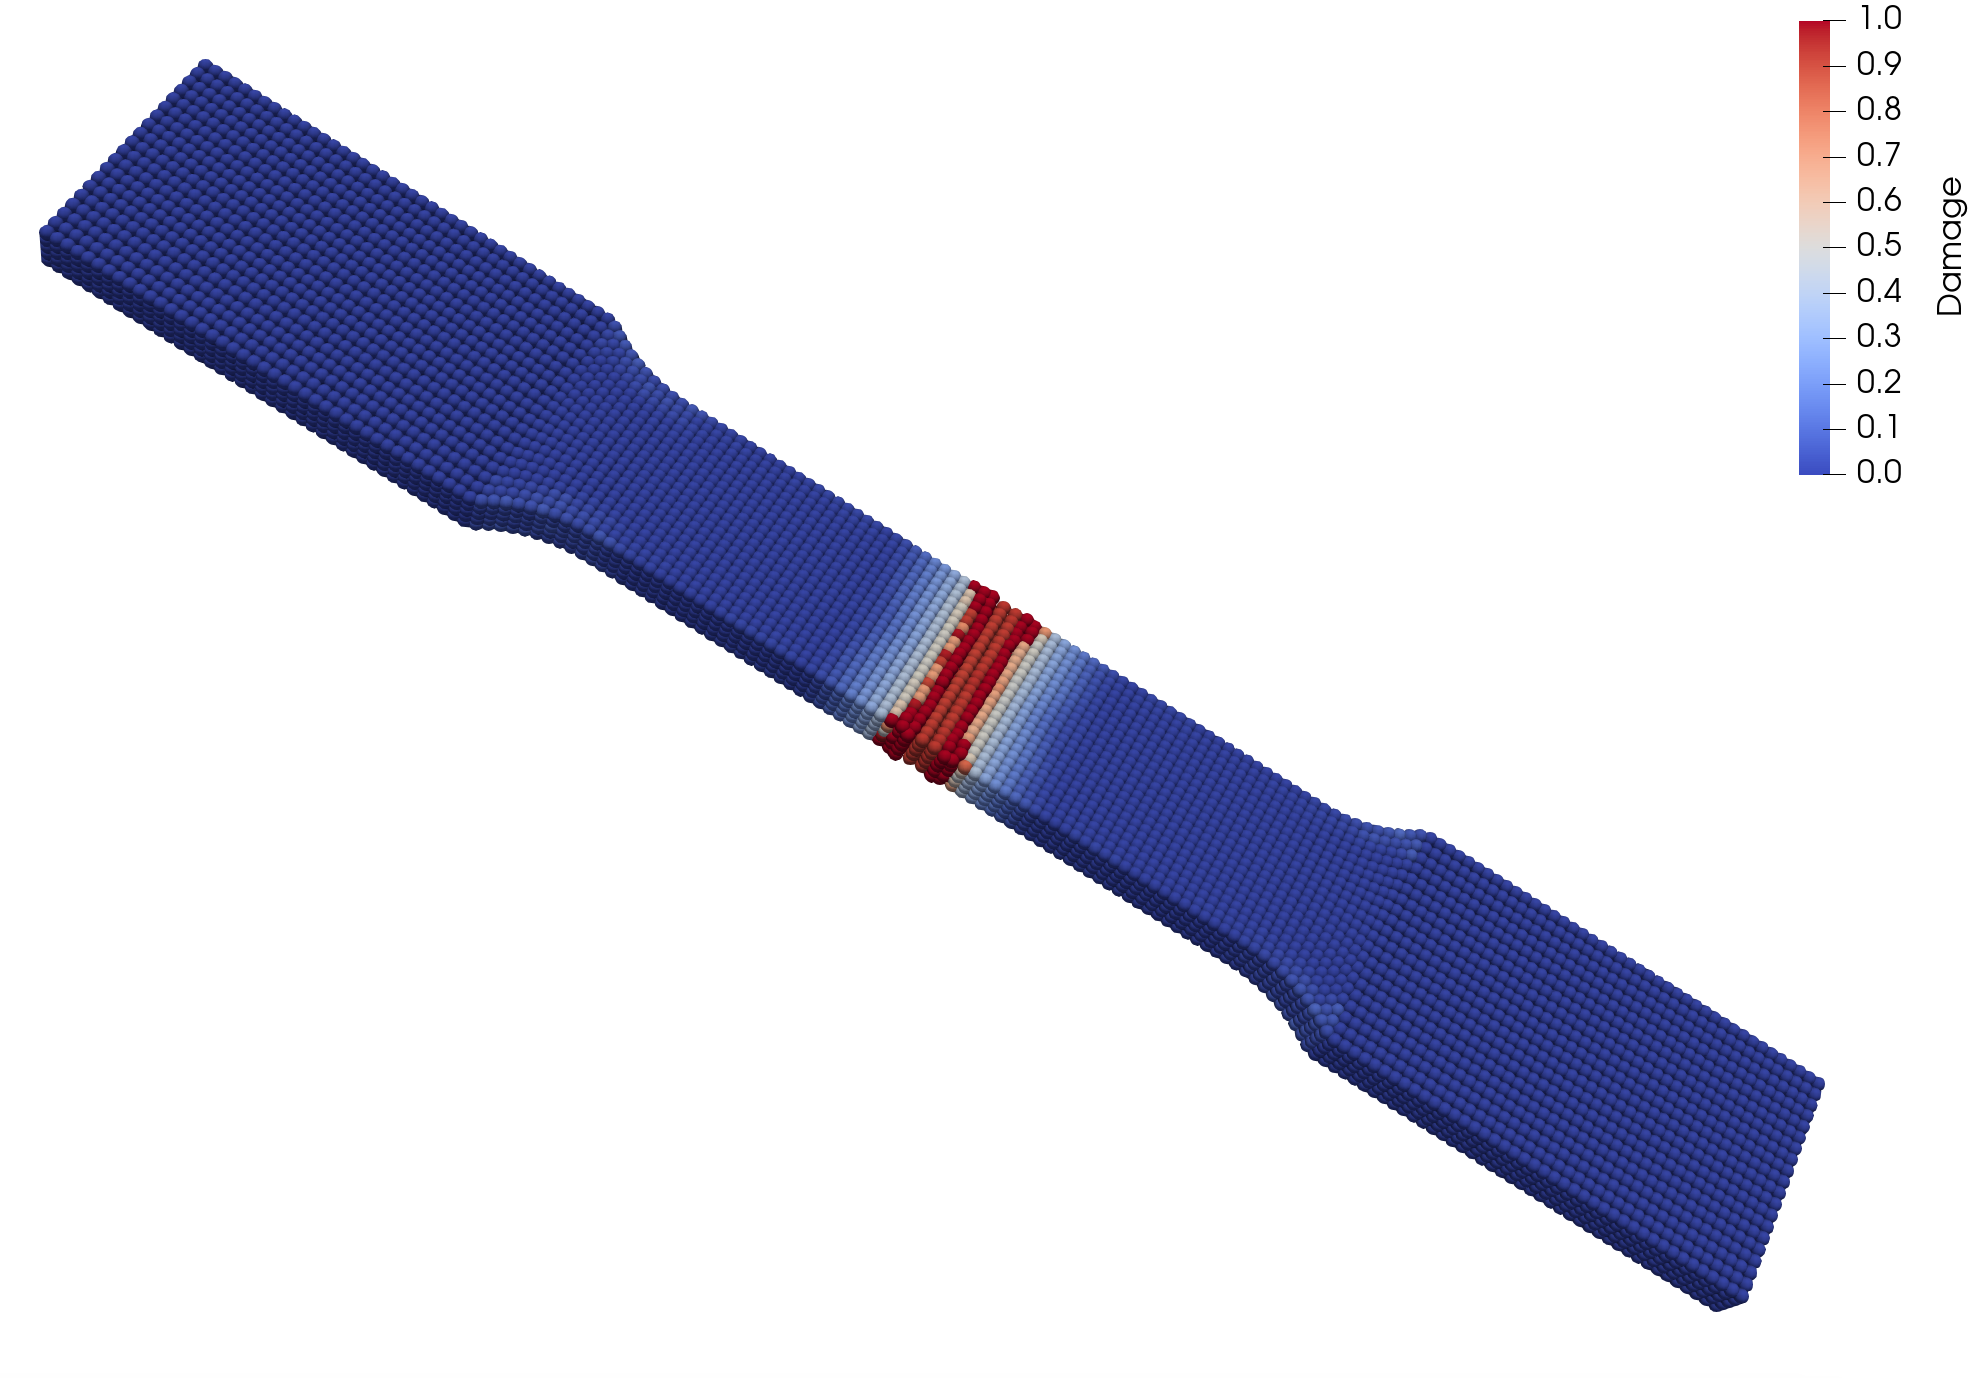
\includegraphics[width=0.9\linewidth]{tensile_test.png}}
\caption{Fracture simulation of tensile tension test with a crack propagating in the middle of the specimen}
\label{fig:tensiletest}
\end{figure}

%=== What is the high-level functionality of Peridynamics.jl? ===%
\texttt{Peridynamics.jl} is an open source Julia \cite{Bezanson2017julia} implementation of peridynamics.
It can be used to conduct simulations with applications such as crack propagation due to external loading conditions (see Fig.~\ref{fig:tensiletest}), or multi-body contact simulations (see Fig.~\ref{fig:logo}).
Users can specify arbitrary geometries as a point cloud to use as a spatial discretization for a simulation.
It is also possible to import meshes generated with ABAQUS and convert them into point clouds.
Multiple peridynamic material models are implemented and can be used in dynamic simulations using Velocity Verlet integration or in quasi-static simulations with an adaptive dynamic relaxation algorithm \cite{Kilic2010}.

%=== What is the purpose of Peridynamics.jl? ===%
The primary purpose of the package is to provide a framework for peridynamic simulations for a broad user base.
Peridynamics simulations can be conducted with custom geometry and setup with just a few lines of code.
Due to Julia's multiple dispatch functionality, custom material models can be defined to extend the package.
Therefore, researchers can use the package to develop new peridynamic material models, simplifying their workflow by utilizing the Julia ecosystem.

\section{Statement of need}
% from the JOSS docs:
% The paper should include a Statement of need section that clearly illustrates the research purpose of the software and places it in the context of related work.

%=== Place the package in the context of related work ===%
The package was already used in numerous publications \cite{Friebertshaeuser2022PAMM,Friebertshaeuser2022AIMS,Partmann2023IJF,Partmann2024AAM,Partmann2024PAMM,Tornquist2022PAMM}.

%=== What is the research purpose of Peridynamics.jl? ===%

\section{Perspectives}


\section{Acknowledgments}
The authors gratefully acknowledge the support of the Deutsche Forschungsgemeinschaft (DFG) in the project \mbox{WE~2525/15-1}.

The authors gratefully acknowledge the support and the supercomputing resources of the Paderborn Center for Parallel Computing (https://pc2.uni-paderborn.de).

% \vadjust{\vfill\pagebreak}

% **************GENERATED FILE, DO NOT EDIT**************

\bibliographystyle{juliacon}
\bibliography{ref.bib}


\end{document}

% Inspired by the International Journal of Computer Applications template
